\documentclass[a4paper,xelatex,ja=standard,fontsize=11pt]{bxjsreport}
\setpagelayout{top=40truemm,bottom=20truemm,left=30truemm,right=30truemm}
\setlength\abovecaptionskip{11pt}

\setCJKmainfont[BoldFont=ToppanBunkyuMidashiMinchoStdN-ExtraBold]{ToppanBunkyuMinchoPr6N-Regular}
\setCJKsansfont[BoldFont=ToppanBunkyuGothicPr6N-DB]{ToppanBunkyuGothicPr6N-Regular}
\setCJKmonofont[BoldFont=ToppanBunkyuGothicPr6N-DB]{ToppanBunkyuGothicPr6N-Regular}
\setmainfont{YuMin-Medium}[LetterSpace=3.0]

\newfontfamily\codefont{FiraCode-Regular}

\usepackage{abstract}
\renewcommand{\abstractnamefont}{\sffamily\bfseries}

\usepackage{tocloft}
\renewcommand\cftchapnumwidth{3.75em}
\renewcommand\cfttoctitlefont{\sffamily\Huge\bfseries}
\renewcommand\cftchapfont{\sffamily\bfseries}

% \usepackage{titlesec}
% \titleformat{\chapter}
%     {\sffamily\huge\bfseries}{\chaptertitlename\ \thechapter\ 章}{1em}{}
% \titleformat{\section}
%     {\sffamily\Large\bfseries}{\thesection}{1em}{}
% \titleformat{\subsection}
%     {\sffamily\large\bfseries}{\thesubsection}{1em}{}
% \titleformat{\subsubsection}
%     {\sffamily\normalsize\bfseries}{\thesubsubsection}{1em}{}

% \usepackage{showframe}
\usepackage{geometry}
\usepackage{url}
\usepackage{listings}

% \usepackage{fancyhdr}
% \pagestyle{fancy}
% \setlength{\headwidth}{\textwidth}
% \addtolength{\headwidth}{3.5truemm}
% \fancyhead{}
% \renewcommand{\chaptermark}[1]{\markboth{第\ \thechapter\ 章~#1}{}}
% \fancyhead[L]{\leftmark}
% \fancyhead[R]{\thepage}
% \fancyfoot{}

\usepackage{tikz}
\usetikzlibrary{arrows.meta}
\usetikzlibrary{trees}
\tikzstyle{every node}=[draw=black,thick,anchor=west]
\tikzstyle{selected}=[draw=red,fill=red!30]
\tikzstyle{optional}=[dashed,fill=gray!50]

\renewcommand{\figurename}{図\;}
\renewcommand{\tablename}{表\;}

\newcommand{\myfootnote}[1]{\,\footnote{#1}\,}
\newcommand{\figref}[1]{図\ref{#1}\;}
\newcommand{\git}{\texttt{Git}}
\newcommand{\gitignore}{\texttt{gitignore}}
\newcommand{\pattern}[1]{{\codefont #1}}

\begin{document}

\begin{titlepage}
	\begin{center}
		\vspace*{\fill}
		\vspace{40pt}
		{\Large 卒業論文}
		\vspace{20pt} \\
		{\huge .gitignoreファイルの実態調査および \\\vspace{10pt} リファクタリング手法の提案} \\
		\vspace{160pt}
		\begin{tabular}{rl}
			{\Large 08232017} & {\LARGE 坂本洸亮}       \\
			\vspace{10pt}                           \\
			{\Large 指導教員}     & {\Large 中丸智貴 \ 助教}  \\
			\vspace{-10pt}                          \\
			                  & {\Large 森畑明昌 \ 准教授}
		\end{tabular}
		\vspace{60pt} \\
		{\Large 2025年1月}
		\vspace{60pt} \\
		{\Large 東京大学教養学部学際科学科総合情報学コース}
		\vspace*{\fill}
	\end{center}
\end{titlepage}

\begin{abstract}
	ここに概要を書く.
\end{abstract}

\newgeometry{top=0truemm,bottom=0truemm}
\setcounter{tocdepth}{2}
\tableofcontents
\thispagestyle{empty}
\restoregeometry

\mainmatter

\pagestyle{headings}
\newgeometry{top=45truemm,bottom=25truemm,left=30truemm,right=30truemm,headsep=10truemm,footnotesep=10truemm}

%
\chapter{はじめに}

バージョン管理システムは,システムやソフトウェアの開発において,ソースコードや関連ファイルの変更履歴を記録し,必要に応じて確認・復元するための機能を提供する.
その中でも\git{}は,高速で効率的なバージョン管理システムとして多くのプロジェクトで採用されている.
\git{}は分散型バージョン管理システムと呼ばれ,リポジトリを一つしか持たない集中型バージョン管理システムに対し,複数のリポジトリを運用するのが特徴である.
メインサーバに配置された共有リポジトリを開発者が各自で複製し,それに対して独立して作業を行った後,それぞれの変更を統合する.
このシステムによって,複数の開発者が並行して作業を行うことが可能となっている.

このようなバージョン管理システムにおいて,管理対象となるファイルを適切に選択することは重要である.
ソースコードやビルドファイルなど,変更履歴を管理する必要があるファイルに対して,バイナリファイルやログファイル,ライブラリを配置するディレクトリなどは管理対象外とすることが一般的である.
これを実現するために,\git{}では\;\texttt{.gitignore}ファイル(以下,単に\gitignore{}と呼ぶ)を用いる.

\gitignore{}は,\git{}の追跡の対象外とするファイルやディレクトリを指定するもので,リポジトリのルートディレクトリに原則配置される.
\git{}は\gitignore{}の各行で指定されたパターンにマッチするファイルやディレクトリを追跡の対象から除外する.
\gitignore{}は,現在追跡されていないファイルやディレクトリが未追跡の状態を保つことを目的とする\cite{git-doc}.
そのため,すでに追跡対象となっているファイルやディレクトリについては\gitignore{}で指定するだけでは除外できず,別途\git{}のインデックスからファイルを除外する必要がある.

\gitignore{}に記述するパターンとして,除外したいファイルやディレクトリのパスをそのまま利用することもできるが,\gitignore{}が提供する機能を活用すれば,より効率的で柔軟な記述が可能となる.
\gitignore{}のパターンで利用できる機能は,メタ文字の形で提供される.
メタ文字は,コンピュータプログラムにおいて特別な意味を持つ文字であり,正規表現など文字列を扱うシステムや,プログラミング言語における引用符など,さまざまな分野・文脈で利用されている.
それ単体で意味を持つものや,隣接する文字に対して作用するもののほか,二つのメタ文字で文字列を囲むことで複数の文字列にマッチさせることができるものなどが存在する.

\gitignore{}においては,正規表現で見られるような文字列のパターンマッチングに利用されるメタ文字のほか,ファイルやディレクトリを扱うための特殊なメタ文字を利用することも可能である.
例として,ディレクトリの区切り文字を表すスラッシュ(\pattern{/})や,
ディレクトリを再帰的にマッチさせるglobstar\myfootnote{GNUによるBash Reference Manual\;\cite{bash-reference}での呼称による.}(\pattern{**})などが挙げられる.

\begin{figure}[h]
	\centering
	\begin{minipage}[c]{0.395\columnwidth}
		\centering
		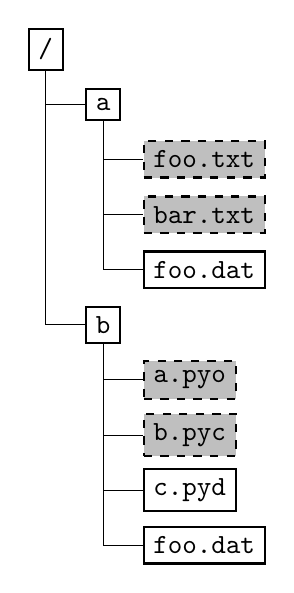
\begin{tikzpicture}[
				node font=\ttfamily,
				grow via three points={one child at (0.5,-0.7) and
						two children at (0.5,-0.7) and (0.5,-1.4)},
				edge from parent path={(\tikzparentnode.south) |- (\tikzchildnode.west)}]
			\node {/}
			child { node {a}
					child { node [optional] {foo.txt}}
					child { node [optional] {bar.txt}}
					child { node {foo.dat}}
				}
			child [missing] {}
			child [missing] {}
			child [missing] {}
			child { node {b}
					child { node [optional] {a.pyo}}
					child { node [optional] {b.pyc}}
					child { node {c.pyd}}
					child { node {foo.dat}}
				};
		\end{tikzpicture}
		\caption{ディレクトリ構造の例}
		\label{fig:gitignore-example-dirtree}
	\end{minipage}
	\begin{minipage}[c]{0.595\columnwidth}
		\centering
		\begin{tikzpicture}[node distance=4cm]
			\node[draw, rectangle, align=center, inner sep=3mm, outer sep=3mm] (from) {
				\lstset{basicstyle=\codefont, breaklines=true}
				\begin{lstlisting}
a/foo.txt
a/bar.txt
b/a.pyo
b/b.pyc
            \end{lstlisting}
			};
			\node[draw, rectangle, align=center, right of=from, inner sep=3mm, outer sep=3mm] (to) {
				\lstset{basicstyle=\codefont, breaklines=true}
				\begin{lstlisting}
a/*.txt
b/?.py[co]
            \end{lstlisting}
			};
			\draw[->, >=Stealth] (from) -- (to);
		\end{tikzpicture}
		\caption{\gitignore{}の記述例}
		\label{fig:gitignore-example}
	\end{minipage}
\end{figure}

例として\figref{fig:gitignore-example-dirtree}のようなディレクトリ構造を考える.
破線で示しているものは,\gitignore{}で除外したいファイルであるとする.
これを実現するような\gitignore{}の記述例を\figref{fig:gitignore-example}に示す.
図左のように除外したいファイルのパスをそれぞれ記述する代わりに,図右のように\gitignore{}の機能を活用することで,より簡潔な記述が可能となる.

このような記述スタイルは,\gitignore{}の記述を簡潔に保つだけでなく,ファイルやディレクトリのパスを抽象化することで,\gitignore{}の保守性や拡張性の向上にも寄与する.
除外対象のファイル名が変更された場合など,\gitignore{}ファイルの修正が必要になった際,それらがパターン化できる限りは既存のパターンの一部を変更するのみでよい可能性が高い.
また,\figref{fig:gitignore-example}の記述に対して,除外する対象として\texttt{a/baz.txt}のようなファイルを追加したい場合,
図右のようなアスタリスク(\pattern{*})を利用した記述により,ディレクトリ\texttt{a}直下の\texttt{.txt}ファイルをすべてマッチさせることができるため,新しい行を追加する必要がなくなる.
このように\gitignore{}の機能を利用することで変更や修正が容易となり,その対象箇所が限定されるため,効率的な保守が可能となるほか,
将来的な除外対象の追加に対応しやすくなり,\gitignore{}の拡張性を向上させることができる.

\begin{figure}
	\centering
	\begin{tikzpicture}[node distance=4cm]
		\node[draw, rectangle, align=center, inner sep=3mm, outer sep=3mm] (variant1) {
			\lstset{basicstyle=\codefont, breaklines=true}
			\begin{lstlisting}
*.txt
*.py[co]
            \end{lstlisting}
		};
		\node[draw, rectangle, align=center, right of=variant1, inner sep=3mm, outer sep=3mm] (variant2) {
			\lstset{basicstyle=\codefont, breaklines=true}
			\begin{lstlisting}
a/*
!a/foo.dat
?.py*
!b/c.pyd
            \end{lstlisting}
		};
		\node[draw, rectangle, align=center, right of=variant2, inner sep=3mm, outer sep=3mm] (variant3) {
			\lstset{basicstyle=\codefont, breaklines=true}
			\begin{lstlisting}
a/*
b/*
!**/foo.dat
!c.pyd
            \end{lstlisting}
		};
	\end{tikzpicture}
	\caption{\gitignore{}の記述の多様性}
	\label{fig:gitignore-example-variants}
\end{figure}

ここで注意すべき点は,機能の利用方法によって同じ結果を与えるパターンが複数存在しうることである.
\figref{fig:gitignore-example-variants}の各記述例は,利用している機能やその利用方法がそれぞれ異なるが,すべて\figref{fig:gitignore-example-dirtree}の状態を実現する.
このような場合,開発者がそれぞれの環境においてどのような記述が最適であるかを判断するためには,\gitignore{}の性質やその機能の十分な理解が必要となる.

このように,\gitignore{}は単にパスを羅列するだけではなく,その機能を活用して幅広い記述が可能である一方,その柔軟性からかえって記述に冗長性や誤りが生じる可能性もある.
ここでいう「冗長性」とは,\gitignore{}の各行について,重複するものが存在したり,ディレクトリ構造的に不要なものが存在することを指す.
誤りは実際の\gitignore{}の挙動で発見することが可能だが,冗長性については各パターンをよく観察する必要があり発見が困難である.

また,\texttt{GitHub}などではさまざまな\gitignore{}のテンプレートが提供されており,リポジトリ作成の際にプロジェクトの種類に応じた\gitignore{}テンプレートを選択することができる.
簡単に\gitignore{}を作成・利用することができる反面,テンプレートは実際のディレクトリ構造や開発環境など,
プロジェクトの状況に適応したものであるとは限らないため,先述したような冗長性が生じやすいと考えられる.

さらに,\texttt{Visual Studio Code}などの統合開発環境(IDE)を利用すると,
新しく除外したいファイルをUIから即座に追加することができるなど,\gitignore{}を直感的かつ簡単に利用することができる.
しかし,このような機能によって,\gitignore{}のアドホックな変更が容易となるうえ,開発者は\gitignore{}の内容を確認することなく変更を行うことになる。

\section{本研究の目的}

\section{本研究の貢献}

\section{関連研究}

%
\chapter{\textrm{gitignore}}

\section{\textrm{gitignore}の各機能の利用状況}

% これの2行目と3行目を入れ替えたときの違い
% a/*
% b/*
% !**/foo.dat
% !c.pyd

\subsection{仮説}

\subsection{検証方法}

\section{\textrm{gitignore}の記述の冗長性・アドホック性}

\subsection{仮説}

\subsection{検証方法}

\section{\textrm{gitignore}とその他の\textrm{ignore}システム}

\subsection{\textrm{ignore}システムの概要}

\subsection{\textrm{ignore}システムで利用されるパターンマッチングシステム}

\subsection{\textrm{gitignore}とその他の\textrm{ignore}システム間での意味論の比較}

%
\chapter{\textrm{gitignore}の各機能の利用状況の調査}

\section{データセットの構築}

\subsection{データの収集}

\subsection{復元処理}

\section{定量分析}

\subsection{手法}

\subsection{結果}

%
\chapter[\textrm{gitignore}のリファクタリングアルゴリズム]{\textrm{gitignore}の\\リファクタリングアルゴリズム}

\section{パターン制約の設計}

\section{アルゴリズムの設計}

\section{アルゴリズムの実装}

\section{アルゴリズムの適用実験}

\subsection{手法}

\subsection{結果}

%
\chapter{考察}

%
\chapter{おわりに}

\backmatter

\begin{thebibliography}{}
	\bibitem{git-doc} Git - gitignore Documentation, \url{https://git-scm.com/docs/gitignore}.
	\bibitem{bash-reference} Bash Reference Manual, \url{https://www.gnu.org/software/bash/manual/bash.html}.
\end{thebibliography}
\clearpage

\end{document}